\section{Method}
\label{sec:method}

The audit has four parts, each answering one question on the setting of
\S\ref{sec:setting}. (1) We compute the SIH criterion for every head
(\S\ref{sec:method-ri}) and (2) the causal importance of every head
(\S\ref{sec:method-causal}), so that the two rankings can be compared without any
head being excluded by construction. (3) We characterize the heads that matter
causally, and the RI-selected heads among them, by where they act, what they read
and what they write (\S\ref{sec:method-char}), and (4) we test how they communicate
and whether the resulting mechanism is faithful (\S\ref{sec:method-circuits}). A
separate analysis across training checkpoints (\S\ref{sec:method-dev}) revisits the
original paper's developmental claim.

\subsection{Reproducing the SIH criterion}
\label{sec:method-ri}

\paragraph{Inputs.}
All 1,024 heads are scored on the 534 discovery prompts (89 families $\times$
base/corrupted/reorder $\times$ two orders). Every fact line, demonstrations
included, is annotated with its head token $t_s$ (the child), tail token $t_o$ (the
mother) and character spans. Since names span several tokens, $t_o$ is anchored at
the first or at the last token of the mother's name; both anchors are reported.

\paragraph{Attention condition.}
Head $h$ qualifies for fact $T$ at current position $j\ge\max(s,o)$ if its actual
attention $A^h_j$, taken from the model's forward pass, satisfies
\begin{equation}
\label{eq:qkgate}
s=\arg\max_{k\le j}A^h_{j,k}
\quad\text{and}\quad
A^h_{j,s} > \tau\max_{k\ne s}A^h_{j,k},
\end{equation}
with the published margin $\tau{=}2.2$. Sensitivity to $\tau$ (the 95th percentile of the observed
dominance ratios is 4.5) is reported in Appendix~\ref{app:stage1}.

\paragraph{Event score.}
For each qualifying $(T,j)$ the score $a^{h,j}_T$ is the clipped, centred share of
the raw-embedding OV projection $x_jW^h_{OV}W_U$ that falls on $t_o$, exactly as in
Appendix~\ref{app:ri}. The index $\mathrm{RI}_h$ is the family-weighted mean of
$a^{h,j}_T$ over events, computed separately for four event populations: all events
(the original pooled index) and, within the test block, events on any test fact or
on the query fact, at any position or at the final answer position.

\paragraph{Controls.}
Each event is paired with the mean score of the other fully visible test-fact
mothers (\emph{name gap}) and of up to three sampled visible non-name word types
(\emph{word gap}). The gaps measure preference for the target relative to these
alternatives; they do not remove a head's static preference for particular tokens
and do not by themselves show that the head represents the relation.

\paragraph{Calibration and selection.}
Two separate procedures follow. A \emph{calibration} tests, on a restricted matched
subset (target and control fully visible, equal in token length, distinct in first
token; at least 50 events in ten families), whether the target is preferred over a
matched alternative under family-consistent label swaps with Holm correction over
all heads. Independently, a \emph{selection rule} fixed before the results ranks
heads descriptively: for each statistic, anchor and event population, the ten
largest positive family-weighted means with at least 20 events in ten families. The
union of these rankings is the \emph{RI-selected} set used in all later
comparisons; membership in it is not a significance claim. Definitions, populations
and sampling policies are given in Appendix~\ref{app:stage1}.

\subsection{Causal importance of every head}
\label{sec:method-causal}

\paragraph{Intervention.}
For head $h$ and a clean/corrupted pair $(x_c,x_r)$, the head's pre-projection
activation $a_h$ (its slice of the input to the attention output projection) on the
clean run is replaced by its value on the corrupted run, and the metric of
Eq.~\ref{eq:metric} is re-read (Figure~\ref{fig:patch}):
\begin{equation}
\label{eq:importance}
I_h = M(x_c) - M\!\left(x_c;\, a_h \leftarrow a_h^{r}\right).
\end{equation}
$I_h>0$ means that the corrupted output of $h$ alone moves the model toward the
corrupted answer. Under Scope~P the replacement covers all original prompt
positions; the two prompts share the demonstrations and the first test fact, so
replacements before the first differing token have no effect, and the patch is
effective on the last 44 of 282 tokens on average. Under Scope~F only the final
colon is replaced. The metric is read at the first divergent answer token in both
scopes; a shared answer prefix is never patched. Scope-F runs store the clean- and
corrupted-answer logits separately, so $I^F_h$ splits into promotion of the
corrupted answer and suppression of the clean one.

\paragraph{Coverage.}
To reduce computation we combine a first-order screen with exact measurements at
two levels of coverage (Table~\ref{tab:coverage}). The screen
\citep{syed2023attribution} estimates every head's importance from one clean
forward, one corrupted forward and one backward pass,
\begin{equation}
\label{eq:screen}
\widehat I_h = -\big\langle \nabla_{a_h} M(x_c),\; a^r_h - a^c_h \big\rangle ,
\end{equation}
a local linear approximation that uses the metric's sensitivity on the clean run
and is obtained for all heads at once. Exact Scope-P patching of \emph{all} 1,024
heads on the 40-pair common subset provides the all-head comparison and calibrates
the screen (pre-registered acceptance: Spearman $\ge 0.7$ against the screen on the
same pairs). Exact Scope-P patching on all 178 pairs is then run for a 148-head
extension set (the screen's top 25, the RI candidates, the heads whose attention at
the answer position selects a test fact, and 25 random controls; composition in
Appendix~\ref{app:stage2}), and Scope-F patching on all 178 pairs for the 69
RI-candidate and answer-position heads. All-head rankings use the common subset
only; extension rankings use the 178 pairs within the extension set; the two are
never mixed. Extension membership was chosen on discovery data before any
measurement outside the common subset.

\begin{table}[t]
\centering\small
\begin{tabular}{@{}lrrl@{}}
\toprule
Measurement & Heads & Pairs & Purpose \\
\midrule
Screen (Eq.~\ref{eq:screen}) & 1,024 & 178 & broad ranking \\
Exact, Scope P & 1,024 & 40 & all-head comparison; calibration \\
Exact, Scope P & 148 & 178 & stable estimates for selected heads \\
Exact, Scope F & 69 & 178 & answer position vs.\ earlier positions \\
\bottomrule
\end{tabular}
\caption{Coverage of the causal map.}
\label{tab:coverage}
\end{table}

\paragraph{Comparisons.}
Effects are averaged over the two orders within a family and then across
families; family-bootstrap intervals are descriptive. The RI selection is compared
with importance in three ways: rank correlation of the RI statistics with $I_h$ (on
the common subset for all heads; within layer as well, since depth affects both);
the share of top-decile heads that lie outside the selection, split by the reason
they were missed; and the median importance of selected heads against the random
controls. Appendix~\ref{app:stage2} gives the pre-registered form of these
criteria.

\begin{figure}[t]
\centering
\resizebox{\columnwidth}{!}{%
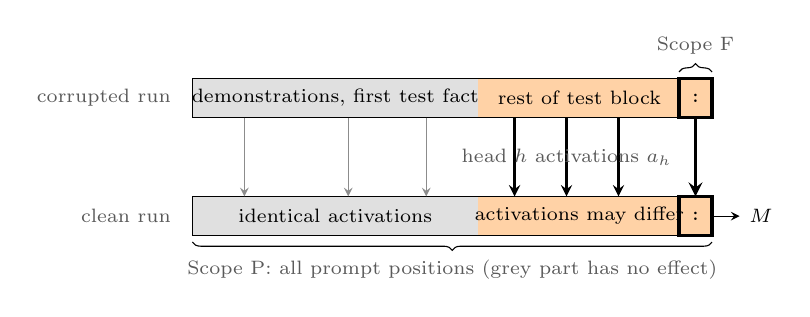
\begin{tikzpicture}[>=stealth, font=\scriptsize]
\def\W{6.6}
% corrupted run
\node[anchor=east, text=black!65] at (-0.15,1.25) {corrupted run};
\fill[black!12] (0,1.0) rectangle (0.55*\W,1.5);
\fill[orange!35] (0.55*\W,1.0) rectangle (\W,1.5);
\draw (0,1.0) rectangle (\W,1.5);
\draw[very thick] (\W-0.42,1.0) rectangle (\W,1.5);
\node at (0.275*\W,1.25) {demonstrations, first test fact};
\node at (0.775*\W-0.2,1.25) {rest of test block};
\node at (\W-0.21,1.25) {\texttt{:}};
% clean run
\node[anchor=east, text=black!65] at (-0.15,-0.25) {clean run};
\fill[black!12] (0,-0.5) rectangle (0.55*\W,0);
\fill[orange!35] (0.55*\W,-0.5) rectangle (\W,0);
\draw (0,-0.5) rectangle (\W,0);
\draw[very thick] (\W-0.42,-0.5) rectangle (\W,0);
\node at (0.275*\W,-0.25) {identical activations};
\node at (0.775*\W-0.2,-0.25) {activations may differ};
\node at (\W-0.21,-0.25) {\texttt{:}};
% arrows: head activations copied
\foreach \x in {0.1,0.3,0.45} {\draw[->, black!45] (\x*\W,1.0) -- (\x*\W,0);}
\foreach \x in {0.62,0.72,0.82} {\draw[->, thick] (\x*\W,1.0) -- (\x*\W,0);}
\draw[->, very thick] (\W-0.21,1.0) -- (\W-0.21,0);
\node[text=black!65] at (0.72*\W,0.5) {head $h$ activations $a_h$};
% braces
\draw[decorate, decoration={brace, amplitude=3pt, mirror}] (0,-0.58) -- (\W,-0.58)
  node[midway, below=3pt, text=black!65] {Scope P: all prompt positions (grey part has no effect)};
\draw[decorate, decoration={brace, amplitude=3pt}] (\W-0.42,1.58) -- (\W,1.58)
  node[midway, above=3pt, text=black!65] {Scope F};
\draw[->] (\W,-0.25) -- ++(0.35,0) node[right] {$M$};
\end{tikzpicture}}
\caption{Single-head activation patching. At a fixed layer, the corrupted run
supplies one head's pre-projection activations to the clean run. Scope~P replaces
all original prompt positions; replacements before the first token difference have
no effect because their activations are identical. Scope~F replaces only the final
colon. The answer contrast is evaluated at the first divergent answer token, leaving
any shared answer prefix unpatched.}
\label{fig:patch}
\end{figure}

\subsection{Characterizing important heads}
\label{sec:method-char}

The causal map says which heads matter and by how much, but not what they do. To
turn a list of heads into hypotheses about a mechanism that Stage~4 can test as
routes and groups, we profile a fixed inventory of 105 heads: every head with a
strong effect on the map, positive or negative, every RI-selected head, a few heads
of moderate effect and the 25 random controls (composition in
Appendix~\ref{app:stage3}). Three questions organize the profile
(Table~\ref{tab:profile}); each is answered per head, and each answer is a
candidate role, not an established one.

\paragraph{Where does the head act?}
Scope-F importance is compared with Scope-P importance, and a single-position scan
patches one test-block position at a time. A head whose effect is confined to the
colon is a candidate \emph{reader}; one whose effect enters at earlier positions is
a candidate \emph{writer}. Neither label follows from the comparison alone: equal
Scope-F and Scope-P effects do not show that the head reads from any particular
position, and single-position effects need not add up to the all-position effect.
Reverse patching, $J_h=M(x_r;\,a_h\leftarrow a^c_h)-M(x_r)$, applies the
intervention in the opposite direction to check its symmetry; recovery is not
assumed and, where found, does not show that one head suffices. The relevance to
the criterion is that the position at which a head's effect enters may differ from
the positions at which it passes the criterion's attention condition or scores
highly on it.

\paragraph{What does it read, and what does it promote?}
At the colon, each head's attention mass is split over the query fact's mother and
child, the distractor mothers and the colon itself, on all prompts rather than only
on events that pass the criterion's gate, so that behaviour the criterion misses is
profiled too. A \emph{changed-query} prompt (the other child is asked about, facts
unchanged) tests whether attention follows the question; reorder and corruption
prompts test whether it follows position. What the head promotes is read from its
actual output vector projected onto the vocabulary, alongside the criterion's
raw-embedding projection of the same position; both are content diagnostics, not
measurements of the effect on the model's output, since a head can act through
later components. Two alternative explanations of a high score are tested directly:
a static preference for repeating tokens (the weight copying score, and whether the
head promotes the name it attends to) and generic induction or retrieval behaviour
(the synthetic probes of \S\ref{sec:rw-readout}). For heads whose effect is
localized to a position that the projections do not explain, a controlled readout
compares the site's residual under the intact head and under a replaced head
activation, with a source-swap control that bounds what the readout can see
(Appendix~\ref{app:stage3}).

\paragraph{What carries the effect?}
At the colon the head's output $A^hV^h$ is recomputed with the attention pattern
$A^h$ and the values $V^h$ taken independently from the clean or the corrupted run.
The two single replacements give a routing term (corrupted pattern, clean values)
and a value term (clean pattern, corrupted values); their sum is compared with the
full patch, and the interaction is reported per family. Whether the values or the
routing dominate is an outcome of this test, not a consequence of the head using
contextual information.

\paragraph{Output of the stage.}
Each head receives a profile: where its effect enters, what it attends to, what its
output promotes, and which alternative explanations apply. The profiles select
components and positions for Stage~4: a head with a localized effect inside a fact
proposes a source position for a route; a later head that attends to that position
proposes a receiver; the routing/value split says which input of the receiver to
test; heads with similar or opposite roles propose groups for redundancy and
interaction tests. Similar profiles are not evidence of a connection. Stage~3
proposes roles and possible connections; Stage~4 tests whether the connections
carry causal effect.

\begin{table}[t]
\centering\small
\setlength{\tabcolsep}{4pt}
\begin{tabular}{@{}p{2.3cm}p{2.5cm}p{2.5cm}@{}}
\toprule
Question & Central test & Use in Stage 4 \\
\midrule
Where does the head act? & Scope F vs.\ P; single-position patches & source and receiver positions \\
What does it read and promote? & query-change control; attention and output profiles & role and connection hypotheses \\
What carries the effect? & attention--value separation & which route input to test \\
\bottomrule
\end{tabular}
\caption{Head profile: questions, central tests and what Stage~4 does with the
answers. Coverage of every measurement is in Appendix~\ref{app:stage3}.}
\label{tab:profile}
\end{table}

\subsection{From heads to a mechanism}
\label{sec:method-circuits}

Stages 2 and 3 measure heads one at a time. The question of the paper is whether
the heads the criterion selects take part in the \emph{mechanism} by which the model
uses a stated relation---heads that pass information to one another, with the
model's MLPs and normalization possibly mediating between them. Stage~3 supplies
the candidates: a localized effect proposes a source position, an attention
profile proposes receivers, and the routing/value split proposes which channel to
test; none of these is yet a connection. Stage~4 asks three questions of them.
All selections use the discovery families; the held-out families are opened once,
for the frozen mechanism.

\paragraph{Communication: which effects between components can be isolated?}
A \emph{route} is a source head, a site, a receiver head and a channel
(Figure~\ref{fig:route}). It is measured in two runs. In a hybrid run, the source's
activation is replaced by its corrupted-run value at the site and the residual
increments of all other components are frozen at their clean values, so that only
the source's change reaches the receiver; the receiver's input on the chosen
channel (keys or values at the site, or its query at the colon) is captured from
this run. In a fresh clean run, the captured channel is injected, only the
receiver's own colon output row changes as a result, and the rest of the model
computes normally to the answer. The change in $M$ is the route effect. A route
shows that the receiver uses what the source wrote, on the declared channel and
against the declared frozen background; it is not an additive share of the
source's total effect, and separately measured routes do not by themselves compose
into a chain. Routes are measured on the 40 common pairs, retained by a fixed
effect-size rule, and the retained ones extended to all 178 pairs in both donor
directions. Sources and receivers come from the Stage-3 profiles and a coverage
check of heads outside the inventory; controls are matched to the type of
intervention (Appendix~\ref{app:stage4}). Where retained routes leave a source's
effect unexplained, a bounded local expansion repeats the measurement with the
MLPs or blocks between source and receiver released rather than frozen; no broad
search over heads is run, and an unresolved source is reported as such.

\paragraph{Joint dependence: how do heads act together, and does a source's
effect need its receivers?}
Retained routes define \emph{groups}: the receivers of one source and the sources
of one receiver. Each group is patched as a whole and minus one member, which gives
the group's nonadditivity $N(S)=I(S)-\sum_{h\in S}I(h)$ and each member's
conditional contribution $\delta_h=I(S)-I(S\setminus\{h\})$. \emph{Receiver
blocking} tests communication in the live model: the source's clean activation is
restored in the corrupted run while its proposed receivers are clamped to their
corrupted outputs; the restoration that is lost measures how much the source's
effect depends on the receivers' response (with self-clamp and reverse controls).
Because of interactions and overlapping paths it is not a partition of the source's
effect into shares. \emph{RI participation} tests the RI-selected heads that pass a
fixed relevance rule (31 heads): each is measured alone, in the intact model and on
a weakened background in which a strong reader has been replaced so that a masked
contribution can show, and the residual RI heads (the 23 without a strong
standalone effect) are compared as a group with layer-matched cohorts of
non-selected heads of the same size. A \emph{backup} test applies the same logic
to a head that moves names strongly but has a negligible standalone effect.
Selected group contrasts are repeated with mean-activation replacement in place of
the corrupted donor, since the baseline changes the strength of group effects.

\paragraph{Explanation quality: does a reduced set of heads preserve the behaviour
and its dependence on facts and query?}
A candidate set $C_0$ is fixed by rule from the strong heads, the coverage
candidates and the RI heads that pass the conditional test. In the \emph{retained}
model (Figure~\ref{fig:retained}) the heads of $C$ stay live at all test-block
positions and the output of every \emph{other head} at those positions is replaced
by its role-matched mean; embeddings, MLPs, normalization, demonstrations and the
answer prefix stay live, so the claim is a head mechanism conditional on the rest
of the model. $C$ is accepted if, family by family, it preserves the model's
clean-minus-corrupted gap, its candidate accuracy in each condition and each order,
and does so more than an all-heads-mean baseline (thresholds in
Appendix~\ref{app:stage4}). The accepted set is \emph{reduced} by removing
pre-declared blocks of heads while the guards hold, and its \emph{completeness} is
checked by removing the same blocks from the full model and from the reduced set
and comparing the losses. Finally, a four-cell panel crosses the fact swap with a
\emph{query change}, with the answer sign held fixed across all four cells, so that
the interaction
\begin{equation}
\label{eq:bd}
B_D=\tfrac14\,\mathbb{E}_{f,o}\!\left[M_D(x_{00})-M_D(x_{10})-M_D(x_{01})+M_D(x_{11})\right]
\end{equation}
measures whether a configuration's answer preference follows the queried binding
rather than the fact swap alone; the
preference and accuracy in each cell are reported alongside it, since a mean
interaction can hide a failing cell. The panel is run on the full model, on the
full model minus the main receiver group and minus the residual RI group, on the
reduced set $C^*$, and on $C^*$ minus its RI members or minus its non-RI members.
The last two test collective dependence on RI-selected heads \emph{inside} the
retained mechanism; they do not show that each member has a relational role or
that the criterion identifies it uniquely. The mask, rosters and thresholds are
frozen before the held-out families are evaluated.

\begin{figure}[t]
\centering
\begin{tikzpicture}[>=stealth, font=\scriptsize, node distance=3pt,
  box/.style={draw, rounded corners=2pt, inner sep=3pt, align=center, minimum width=3.3cm},
  zone/.style={draw, dashed, rounded corners=3pt, inner sep=5pt},
  lab/.style={text=black!65}]
\node[box, fill=orange!35] (S) at (0,0) {source replaced at its site;\\other increments frozen};
\node[box, below=of S] (C) {receiver channel captured\\(K/V at site, or Q at colon)};
\node[zone, fit=(S)(C), label={[lab]above:1. perturb the channel (hybrid run)}] (Z1) {};
\node[box, fill=black!6, below=0.55cm of C] (I) {channel injected into a clean run;\\receiver's colon output changes};
\node[box, below=of I] (M) {rest of the model computes normally\\$\rightarrow$ $M$};
\node[zone, fit=(I)(M), label={[lab]above:2. measure the effect (fresh run)}] (Z2) {};
\draw[->, thick] (S) -- (C);
\draw[->, thick] (C) -- (I);
\draw[->, thick] (I) -- (M);
\end{tikzpicture}
\caption{A route. Zone 1: the source is replaced and all other residual increments
are frozen, so the receiver's channel reflects only the source's change. Zone 2:
the captured channel is injected into a fresh clean run; the receiver's colon output
changes and the rest of the model runs normally to the answer.}
\label{fig:route}
\end{figure}

\begin{figure}[t]
\centering
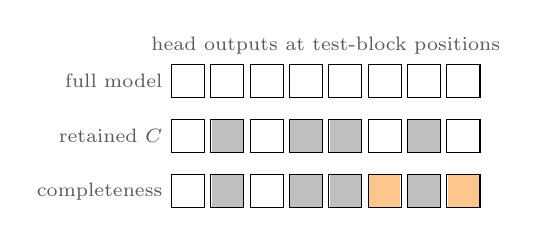
\begin{tikzpicture}[>=stealth, font=\scriptsize,
  head/.style={draw, minimum width=0.42cm, minimum height=0.42cm, inner sep=0pt},
  lab/.style={text=black!65}]
\foreach \r/\name in {0/full model, 1/retained $C$, 2/completeness} {
  \node[lab, anchor=east] at (-0.2,-\r*0.7) {\name};
  \foreach \i in {0,...,7} {\node[head] (h\r\i) at (\i*0.5,-\r*0.7) {};}
}
\foreach \i in {1,3,4,6} {\fill[black!25] ([shift={(-0.2,-0.2)}]h1\i.center) rectangle ++(0.4,0.4);}
\foreach \i in {1,3,4,6} {\fill[black!25] ([shift={(-0.2,-0.2)}]h2\i.center) rectangle ++(0.4,0.4);}
\foreach \i in {5,7} {\fill[orange!45] ([shift={(-0.2,-0.2)}]h2\i.center) rectangle ++(0.4,0.4);}
\node[lab] at (1.75,0.45) {head outputs at test-block positions};
\end{tikzpicture}
\caption{The retained-mechanism test. Only head outputs at test-block positions are
intervened on. White: head live. Grey: head output replaced by its role-matched
mean. Orange: a block removed for the completeness check, removed identically from
the full model. MLPs, normalization, embeddings, demonstrations and the answer
prefix are live in every configuration.}
\label{fig:retained}
\end{figure}

\subsection{Developmental check}
\label{sec:method-dev}

The second gap of \S\ref{sec:sih} concerns training: \citet{ren2024semantic} infer
that SIHs drive the emergence of in-context learning from the co-timing of a
behavioural transition with rising indices in heads selected because their index
rises. We run an adapted version of that analysis on OLMo-2's public pre-training
checkpoints: not a replication of the original emergence point, which a different
model, training run and preprocessing can shift, but a test of the same
developmental relation inside our model.

\paragraph{Design.}
Behaviour is measured as in the original, with the same four synthetic
classification task families, the same shot ladder and the same distinction
between format compliance and pattern discovery; accuracy is constrained to the
legal task labels, and format validity is checked separately against the
vocabulary-wide top token. Fifty frozen prompts per task and shot count are reused
at every checkpoint (17 checkpoints, 1B--3.9T tokens), so comparisons are paired.
The relation index is computed for all 1,024 heads at ten of these checkpoints on
700 balanced AGENDA relation triplets, with the original developmental gate (source
token is the attention argmax) as primary and the full $\tau{=}2.2$ gate as
sensitivity. Two additions go beyond the original. First, alongside the index over
gated events, we record how often the gate passes and the index per measurement
opportunity, in which events that fail the gate contribute zero; a developmental
change can then be located in routing frequency or in selectivity among routed
events. Second, instead of following selected rising curves, the heads with the
highest index at the final checkpoint are traced backwards and the overlap between
each checkpoint's top heads and the final set is measured, which tests whether the
early and the mature high-index heads are the same heads. The broad behavioural
window was fixed before the index timing was analysed; three checkpoints inside it
were added to the behavioural measurement after a routing peak had been seen in the
index, and the results keep the two apart (Appendix~\ref{app:dev}).
